\documentclass[11pt]{article}

\usepackage[margin=1in]{geometry}
\usepackage{fancyhdr}

\pagestyle{fancy}

\lhead{Multi-Agent Path Optimization} \rhead{\today}
\renewcommand{\headrulewidth}{0.4pt}
\setlength{\headheight}{13.6pt}

\usepackage{csquotes}
\usepackage{amsmath}

\usepackage{graphicx}
\graphicspath{{figs}}
\usepackage[justification=centering]{caption}

\usepackage{xcolor}
\definecolor{navy}{HTML}{2F729C}
\colorlet{linkcolor}{navy}

\usepackage[linktoc=all,colorlinks,allcolors=navy]{hyperref}
\usepackage[nameinlink]{cleveref}

%\usepackage{biblatex}
%\addbibresource{references.bib}

\usepackage{lipsum}
\usepackage{xcolor}

\usepackage[toc,page]{appendix}
\usepackage{tocloft}
\renewcommand{\cftsecleader}{\cftdotfill{\cftdotsep}}

\usepackage{enumitem}
\setlist{  
	listparindent=\parindent,
	parsep=0pt,
}

\usepackage{listings}
\usepackage{matlab-prettifier}

\definecolor{light-gray}{gray}{0.95}
\lstnewenvironment{matlab}{
	\lstset{backgroundcolor=\color{light-gray}}
	\lstset{language=matlab}
	\lstset{style=Matlab-Pyglike}
	\lstset{numbers=left}
	\lstset{frame=single}
	\lstset{basicstyle=\ttfamily\footnotesize}
}{}
\usepackage{amsmath}
\usepackage{amsthm}
\usepackage{amssymb}
\usepackage{amsfonts}
\usepackage{mathtools}
\usepackage{multirow}
\usepackage{multicol}
\usepackage{stackrel}
\usepackage{titlesec}
\usepackage{comment}

\begin{comment}
\usepackage[T1]{fontenc}
\usepackage{charter}
\usepackage[charter]{mathdesign}    
\end{comment}
  
% some macros
\newcommand{\set}[1]{\{ #1 \}}
\newcommand{\Bigset}[1]{\Big\{ #1 \Big\}}
\newcommand{\mat}[4]{\begin{bmatrix} #1 & #2 \\ #3 & #4 \end{bmatrix}}
\newcommand{\conj}[1]{\bar{#1}}
%\DeclareMathOperator{\dim}{dim}
\DeclareMathOperator{\im}{im}
\DeclareMathOperator{\nullity}{nullity}
\DeclareMathOperator{\tr}{trace}
\DeclareMathOperator{\rank}{rank}
\DeclareMathOperator{\fcn}{fcn}
\DeclareMathOperator{\Var}{Var}
\DeclareMathOperator{\var}{var}
%\DeclareMathOperator{\sp}{Span}
%\DeclareMathOperator{\det}{det}
\newcommand{\R}{\mathbb{R}}
%\newcommand{\B}{\mathcal{B}}
\newcommand{\C}{\mathbb{C}}
\newcommand{\Z}{\mathbb{Z}}
\newcommand{\N}{\mathbb{N}}
\newcommand{\Q}{\mathbb{Q}}
\renewcommand{\P}{\mathbb{P}} % for probability measure
\renewcommand{\sp}{\text{Span}}
%\renewcommand{\CC}{\textbf{C}}
%\renewcommand{\S}{\mathcal{S}}
\newcommand{\M}{\mathbb{M}}
\newcommand{\al}{\alpha}
\newcommand{\be}{\beta}
%\newcommand{\p}{\varphi}
\newcommand{\ga}{\gamma}
\newcommand{\la}{\lambda}
\newcommand{\eps}{\varepsilon}
\renewcommand{\th}{\theta}
\newcommand{\sse}{\subseteq}
\newcommand{\dd}{\, \mathrm{d}}
\renewcommand{\d}{\mathrm{d}}
\newcommand{\dual}{^*}
\newcommand{\orth}{^{\perp}}
%\renewcommand{\c}{^{\text{c}}}
\newcommand{\lV}{\lVert}
\newcommand{\rV}{\rVert}
\newcommand{\V}{\Vert}
\newcommand{\lv}{\lvert}
\newcommand{\rv}{\rvert}
\renewcommand{\v}{\vert}
\newcommand{\lan}{\left\langle}
\newcommand{\ran}{\right\rangle}
\newcommand{\dir}{\oplus}
\newcommand{\ang}[1]{\left\langle #1 \right\rangle}
\newcommand{\abs}[1]{\left\lvert #1 \right\rvert}
\newcommand{\norm}[1]{\left\lVert #1 \right\rVert}
\newcommand{\adj}{^*}
\newcommand{\blankang}{\ang{\phantom{v},\phantom{v}}}
\renewcommand{\i}{\sqrt{-1}}
\newcommand{\ds}{\displaystyle}
\newcommand{\dsum}{\displaystyle\sum}
\newcommand{\dprod}{\displaystyle\prod}
\DeclareMathOperator{\cis}{cis}
\newcommand{\an}{^0}
%\DeclareMathOperator{\inf}{inf}
%\DeclareMathOperator{\sup}{sup}
\renewcommand{\sp}{\,\,}
\newcommand{\ex}{\exists \,}
\newcommand{\fa}{\forall}
\renewcommand{\l}{\ell}
\newcommand{\overbar}[1]{\mkern 1.5mu\overline{\mkern-1.5mu#1\mkern-1.5mu}\mkern 1.5mu} % custom overline that is slightly smaller
\newcommand{\cl}[1]{\overbar{#1}}
\newcommand{\seq}[1]{\set{#1}_{n\geq 1}}
\newcommand{\dcup}{\displaystyle\bigcup}
\newcommand{\dcap}{\displaystyle\bigcap}
\newcommand{\dliminf}{\displaystyle\liminf}
\newcommand{\dlimsup}{\displaystyle\limsup}
\newcommand{\dlim}{\displaystyle\lim}
\newcommand{\ndlim}{\displaystyle\lim_{n \to \infty}}
\newcommand{\mdlim}{\displaystyle\lim_{m \to \infty}}
\newcommand{\Ndlim}{\displaystyle\lim_{N \to \infty}}
\newcommand{\dint}{\displaystyle\int}
\renewcommand{\qed}{\hfill $\square$}
\newcommand{\evan}{$\phantom{evan}$ \qed}
\newcommand{\kotha}{\dsum_{n=0}^{\infty}}
\newcommand{\kothaa}{\dsum_{n=1}^{\infty}}
\DeclareMathOperator{\sgn}{sgn}
\newcommand{\minus}{\hspace{1pt}\texttt{\char`\\}\hspace{1pt}}
\newcommand{\ba}{\mathbf{a}}
\newcommand{\bb}{\mathbf{b}}

\usepackage{mathrsfs}

\newcommand{\Y}{\mathscr{Y}} % C^1 function vector space
\newcommand{\D}{\mathscr{D}} % domain of functions

% for 2-d vectors
\newcommand{\x}{\mathbf{x}}
\newcommand{\y}{\mathbf{y}}
\newcommand{\z}{\mathbf{z}}
\renewcommand{\c}{\mathbf{c}}
\newcommand{\p}{\mathbf{p}}

\usepackage[symbol]{footmisc}
\usepackage[numberedsection,symbols,nogroupskip,sort=none]{glossaries-extra}

\glsxtrnewsymbol[description={number of robots}]{N}{\ensuremath{N}}
\glsxtrnewsymbol[description={number of circular obstacles}]{M}{\ensuremath{M}}
\glsxtrnewsymbol[description={initial position of the \(i\)-th robot}]{x_i}{\ensuremath{\x_i}}
\glsxtrnewsymbol[description={target position of the \(i\)-th robot}]{y_i}{\ensuremath{\y_i}}
\glsxtrnewsymbol[description={path of the \(i\)-th robot}]{p_i}{\ensuremath{\p_i}}
\glsxtrnewsymbol[description={radius or repulsive distance of robots}]{r}{\ensuremath{r}}
\glsxtrnewsymbol[description={center of the \(j\)-th circular obstacle}]{c_j}{\ensuremath{\c_j}}
\glsxtrnewsymbol[description={radius of circular obstacles}]{R}{\ensuremath{R}}
\glsxtrnewsymbol[description={objective function}]{F}{\ensuremath{F}}
\glsxtrnewsymbol[description={Lagrangian function}]{L}{\ensuremath{L}}
\glsxtrnewsymbol[description={barrier function}]{g}{\ensuremath{g}}

\begin{document}

\begin{titlepage}
    \centering
    \null
    \vspace{\stretch{1}}
    
    {\huge \textbf{Multi-Agent Path Optimization\\using Calculus of Variations}\par}
    \vspace{5mm}
    {\Large \large Course Project\par
    MATH 146 --- Methods of Applied Mathematics\par}
    \vspace{5mm}
    {\large \textbf{Author:} Robert Lee and Vedant Yogishwar\par
    \textbf{Instructor:} Dr. Shiba Biswal\par}
    
    \vspace{\stretch{2}}
    
    {\large \today\par}
\end{titlepage}

\clearpage

\tableofcontents

\clearpage

\begin{abstract}
\lipsum[1-2]
\end{abstract}

\clearpage

\printunsrtglossary[type=symbols,style=long,title={List of Symbols}]

\section{Introduction}

\section{Theory}
\underline{\textbf{The Secant Method: Basic Description}}
In simple terms, the secant method is an iterative method that—through initial guesses—formulates a sequence of approximations layered onto each other. Based on the principles of a root-finding algorithm, the workings of this model relay the chosen initial guesses through a function (as seen in the following description) which allows the algorithm to predict the next iterative term. This term is then subjected to the same equation, formulating a recurrence relation until the desired level of accuracy is achieved. In the simple case of two initial conditions x_0 and x_1, the next iterative term in this model is given by 
\begin{equation}
x_2 = x_1 - \frac{f(x_1) \cdot (x_1 - x_0)}{f(x_1) - f(x_0)}
\end{equation}

\subsection{Problem Definition}

\textcolor{red}{Add description of problem here.}

Let \(\p_i \in C^1([0,1])^2\) be the vector valued function corresponding to the path of the \(i\)-th robot. Then we have that \(\p_i(0) = \x_i\) and \(\p_i(1) = \y_i\). The length of the path is defined as
\begin{equation}
    l_i = \int_0^1 \norm{\p_i'(t)}^2 dt.
\end{equation}

\subsection{Objective Function}

We wish to minimize the total length of all robot paths. Define \(F\) as the total path length
\begin{equation}
    F(P) = \int_0^1 \sum_{i=1}^{N} \norm{\p_i'(t)}^2 dt,
\end{equation}
where \(P = [\p_1, \ldots, \p_N]^\intercal\) is the path ensemble.

We will modify the objective function in order to represent the no-collision and obstacle constraints. As an example, consider the obstacle constraint. In order to check whether or not a robot collides with an obstacle, a function \(g\) can be defined such that it evaluates to infinity if the distance between the robot and the center of the obstacle is less than \(R\) and evaluates to 0 when not. However, \(g\) would be discontinuous and forbid the use of calculus of variations techniques.

A barrier function \(g_{d,\mu}\) is a continuous function that goes to infinity as it approaches a ``barrier'' value \(d\). A parameter \(\mu\) can be varied in order for \(g\) to approach the discontinuous form. In this case, we wish to devise a function that goes to infinity when approached from above to act as a repulsor. In this project, we will consider two types of barrier functions
\begin{enumerate}
    \item Log function:
    \begin{equation}
        g_{d,\mu}(x) = \frac{-1}{\mu} \log(x-d),
        \quad
        g'_{d,\mu}(x) = \frac{-1}{\mu(x-d)}.
    \end{equation}
    \item Inverse function:
    \begin{equation}
        g_{d,\mu}(x) = \frac{1}{\mu(x-d)},
        \quad
        g'_{d,\mu}(x) = \frac{-1}{\mu(x-d)^2}.
    \end{equation}
\end{enumerate}

Using this barrier function we can rewrite \(F\) as
\begin{equation}
    F(P) = \int_0^1 \left[ \sum_{i=1}^{N} \norm{\p'_i(t)}^2 + \sum_{i,j = 1; i \neq j}^{N} g_{r,\mu_1}\left( \norm{\p_i(t) - \p_j(t)}^2 \right) + \sum_{i=1}^{N} \sum_{j=1}^{M} g_{R,\mu_2}\left( \norm{\p_i(t) - \c_j}^2 \right) \right] dt,
\end{equation}
and the optimization problem becomes an unconstrained optimization problem.

\subsection{First-Order Necessary Conditions}

To derive first-order necessary condition, we first identify the Lagrangian \(L\),
\begin{equation}
    L(Y,Z) = \sum_{i=1}^{N} \norm{\z_i}^2 + \sum_{i,j = 1; i \neq j}^{N} g_{r,\mu_1}\left( \norm{\y_i - \y_j}^2 \right) + \sum_{i=1}^{N} \sum_{j=1}^{M} g_{R,\mu_2}\left( \norm{\y_i - \c_j}^2 \right).
\end{equation}
Applying the Euler--Lagrange equation w.r.t.\ the \(x\)-component of the \(i\)-th robot,
\begin{equation}
    \frac{d}{dt}\left(\p'_{i,x}\right) = \sum_{j \neq i} g'_{r,\mu_1}\left( \norm{\p_i - \p_j}^2 \right) (\p_{i,x} - \p_{j,x}) + \sum_{j=1}^{M} g'_{R,\mu_2}\left( \norm{\p_i - \c_j}^2 \right) (\p_{i,x} - \c_{j,x}).
    \label{eq:EL}
\end{equation}
An analogous equation can be derived w.r.t.\ its \(y\)-component by replacing \(x\) with \(y\).

\subsection{Differential Equation}

The Euler-Lagrange equation derived in \Cref{eq:EL} provides a system of differential equations that govern the motion of each robot's path.

\section{Cases}

\subsection{Validating Obstacle Avoidance}

In order to validate the transformation of the constrained optimization problem into an unconstrained one, we consider the simplest possible case that exhibits all phenomena in the system: two robots and one obstacle. It has the parameters
\begin{align*}
	\x_1 = (-50,-20),\,\y_1 = (50,20),\,\x_2 = (50,-20),\,\y_2 = (-50,20),\,\c_1 = (0,0),\, \text{and } R = 10.
\end{align*}
The initial and target positions of the two robots are placed such that if they travel in a straight line, they will cross each other at the origin and create the shape of an X. At this intersection, a circular obstacle is placed.

The soft-penalty tuning parameters are set to \(\mu_1 = 10^{-3}\), \(r = 0\), and \(\mu_2 = 5 \times 10^{-4}\). We set a small robot radius and make the effect of the obstacle double that of the robots themselves. This is because the obstacle is the dominant force in the scenario.

A manual ``guess-and-check'' shooting scheme is used. The initial velocity is set to aim tangent below and above for robot 1 and 2, respectively, with a magnitude of \(\sqrt{100^2 + 40^2} \approx 107.7\)---which is the distance both robots must travel if they move in a straight line. This is further tuned to produce the trajectory in \Cref{fig:n2m1-paths}.

\begin{figure}
	\centering
	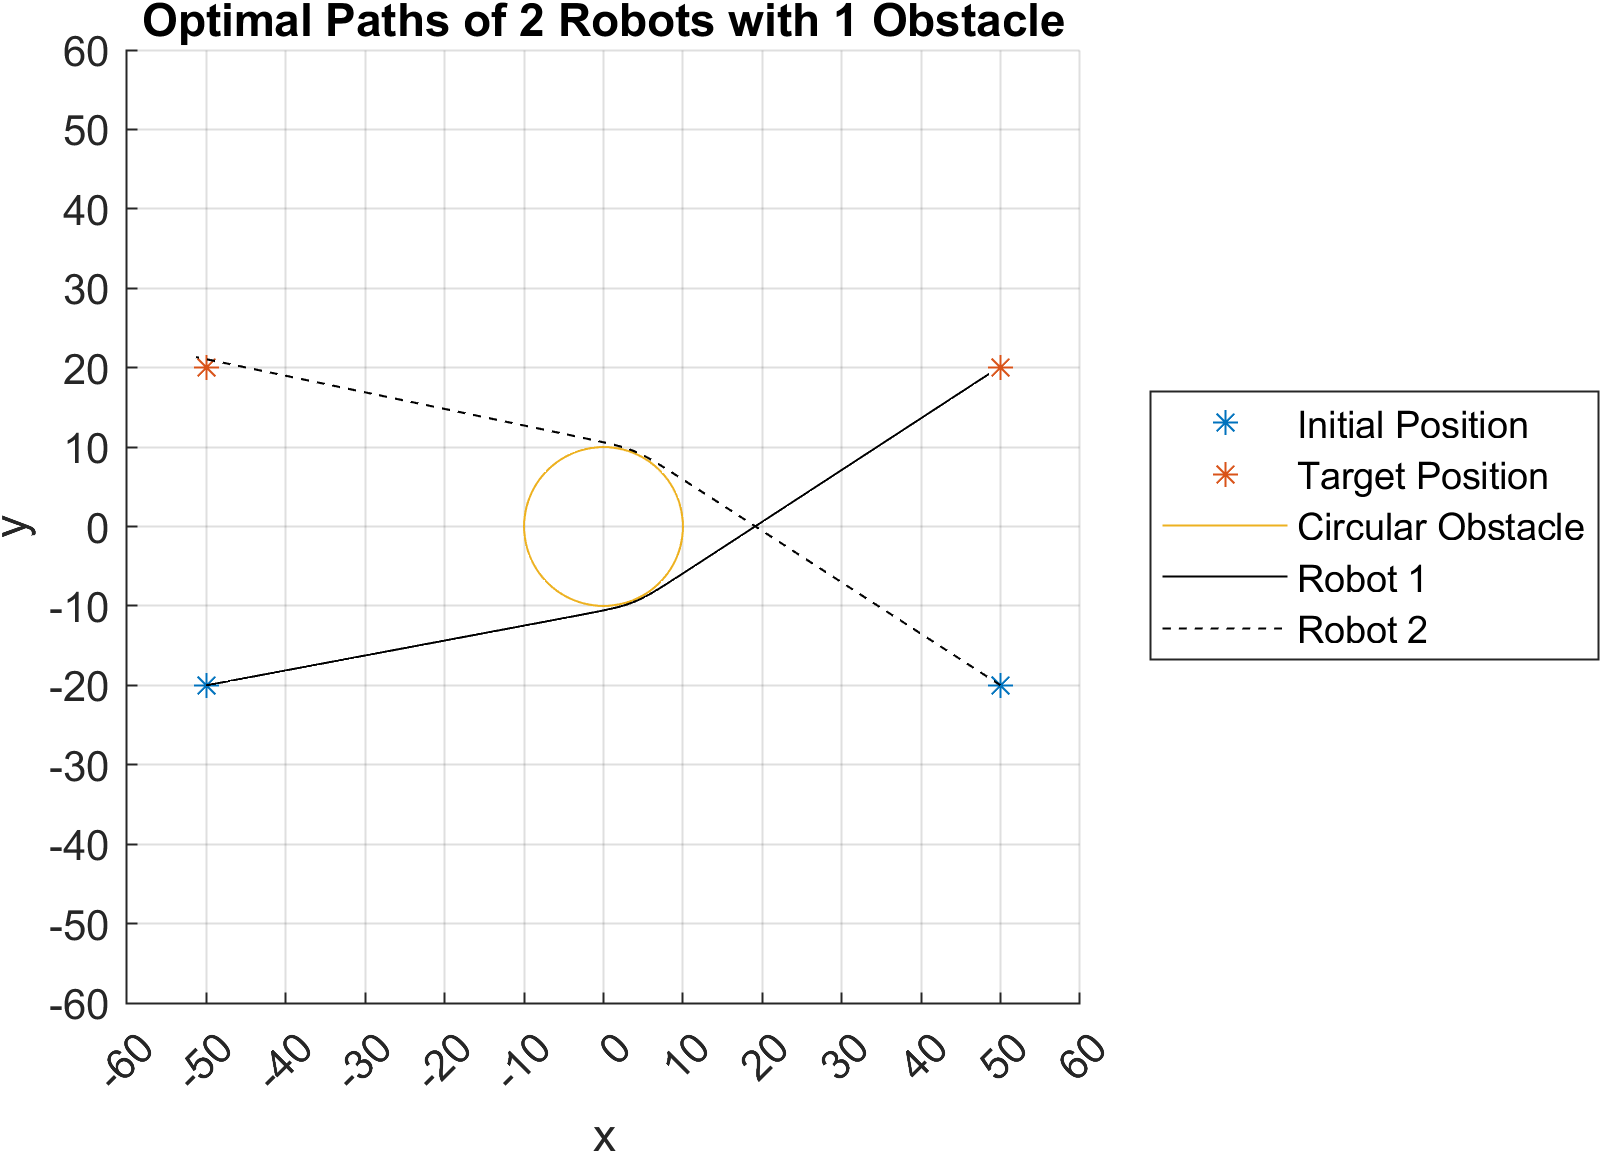
\includegraphics[width=0.75\linewidth]{N2M1_paths}
	\caption{Optimal trajectories for two robots and one obstacles placed in an X shape. The trajectories were found by a manual shooting scheme.}
	\label{fig:n2m1-paths}
\end{figure}

A shooting scheme algorithm that used the secant method was attempted, but convergence did not occur due to the sensitivity of the barrier function used. A small change in initial condition could result in the trajectory hitting the obstacle, which would cause \texttt{ode45} to fail and terminate early---before reaching time \(t = 1\).

\subsection{More Robots}

Due to the sensitivity of obstacles, we decided to investigate the efficacy of the secant method with only robot repulsion. 10 robots were used in the first case and their initial and target positions were uniformly and randomly placed within the cell \([-100,100] \times [-100,100]\).

As the secant method must be seeded by two initial guesses, the following scheme was used. For the first initial guess, a velocity direction was chosen, for each robot, uniformly at random from \(0\) to \(2\pi\). The magnitude of its initial velocity was set to the distance between its initial position and target position. The second initial guess perturbed each robot's velocity direction by up to 1 degree. This was chosen as it would allow for a relatively smooth approximation of the derivative, as opposed to two diametric initial velocity guesses.

50 iterations were used to find the optimal trajectory shown in \Cref{fig:n10m0-paths}. We can see the repulsive effect between robots in the curved trajectory of the robot moving from \(\sim(-60,20)\) to \(\sim(-80,40)\), which is caused by the influence of the robot southwest of it. \Cref{fig:n10m0-paths-zoom} shows a zoomed in section of the domain where two paths cross and turn to reach the target position.

\begin{figure}
	\centering
	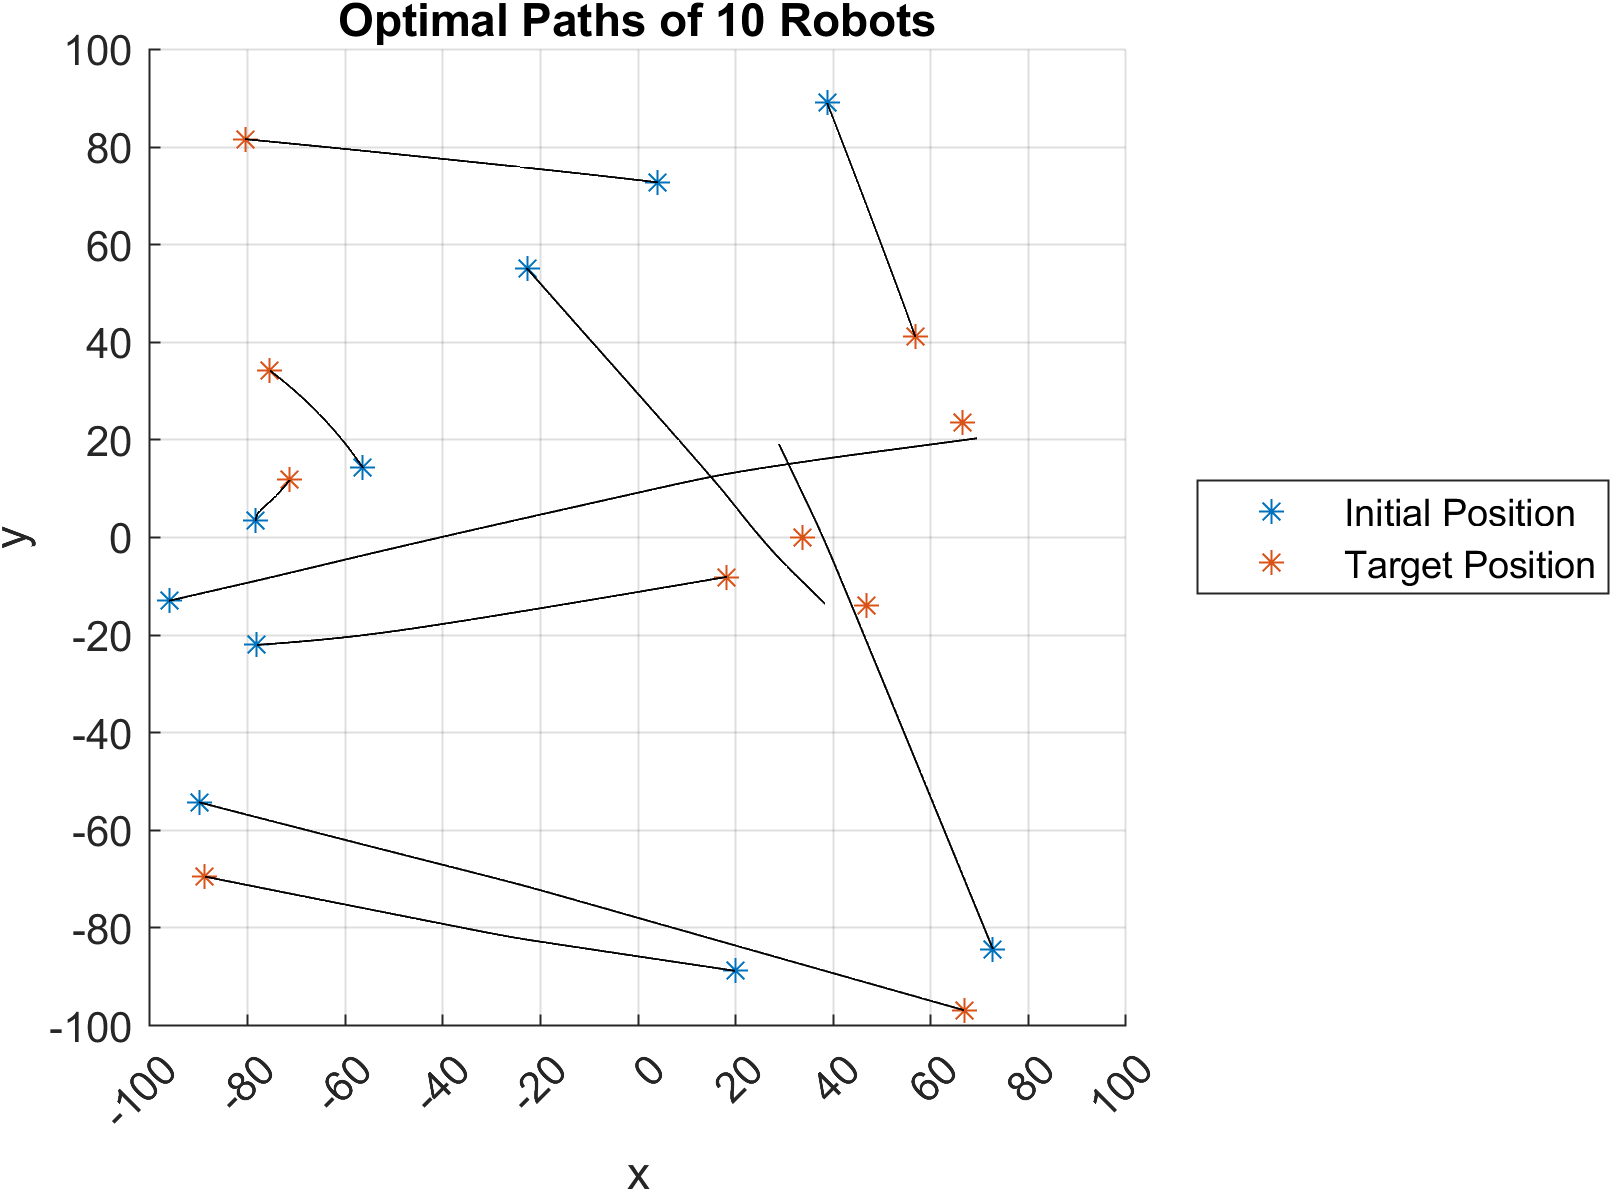
\includegraphics[width=0.75\linewidth]{N10M0_paths}
	\caption{Optimal trajectories for 10 robots and no obstacles placed uniformly at random. The trajectories were found using a shooting algorithm with the secant method.}
	\label{fig:n10m0-paths}
\end{figure}

\begin{figure}
	\centering
	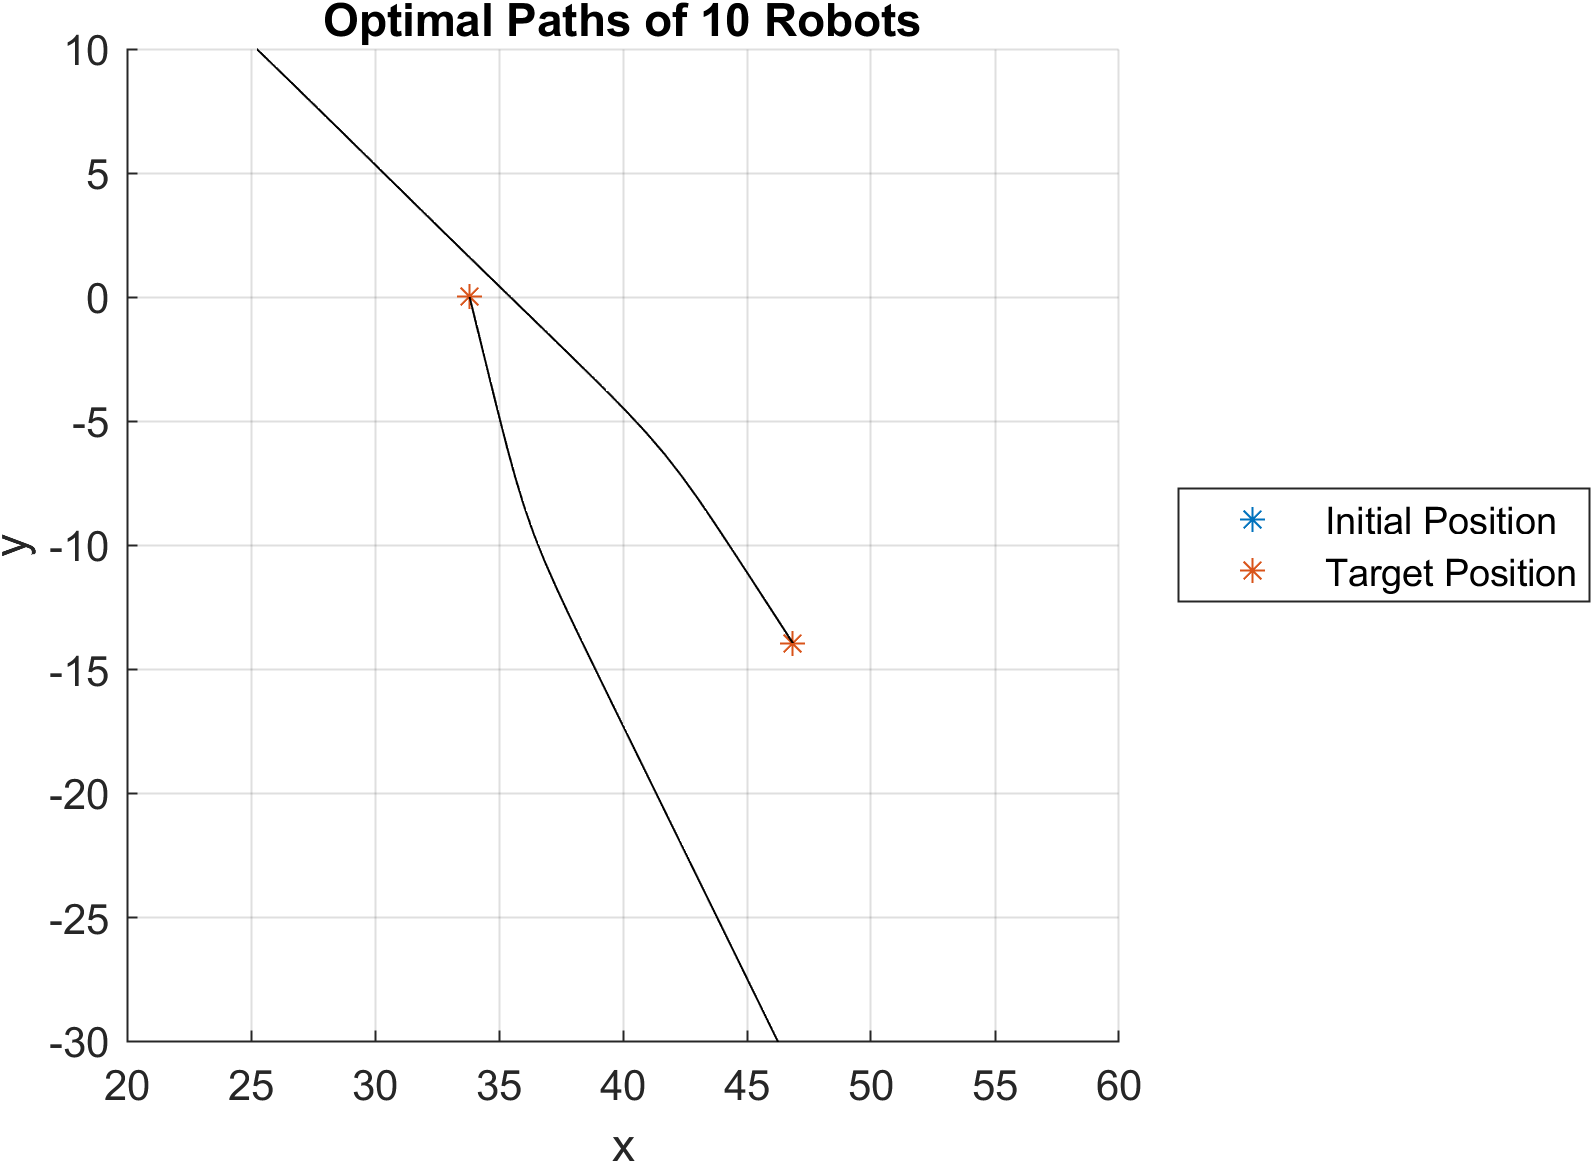
\includegraphics[width=0.75\linewidth]{N10M0_paths_zoom}
	\caption{The region \([20,60] \times [-30,10]\) in \Cref{fig:n10m0-paths}. The curvature of the path can clearly be seen from two target positions.}
	\label{fig:n10m0-paths-zoom}
\end{figure}

\clearpage

The convergence of the secant method can be seen in \Cref{fig:n10m0-t-err}. A high rate of convergence can been seen from iteration 0 to 10--15, from where it slows down slightly. Great convergence can be seen, with an average target position error of \(\sim 10^{-6}\) for each robot. The distribution of target position errors is shown in \Cref{fig:n10m0-p-err} with all trajectories ending less than \(10^{-5}\) from their target position.

\begin{figure}
	\centering
	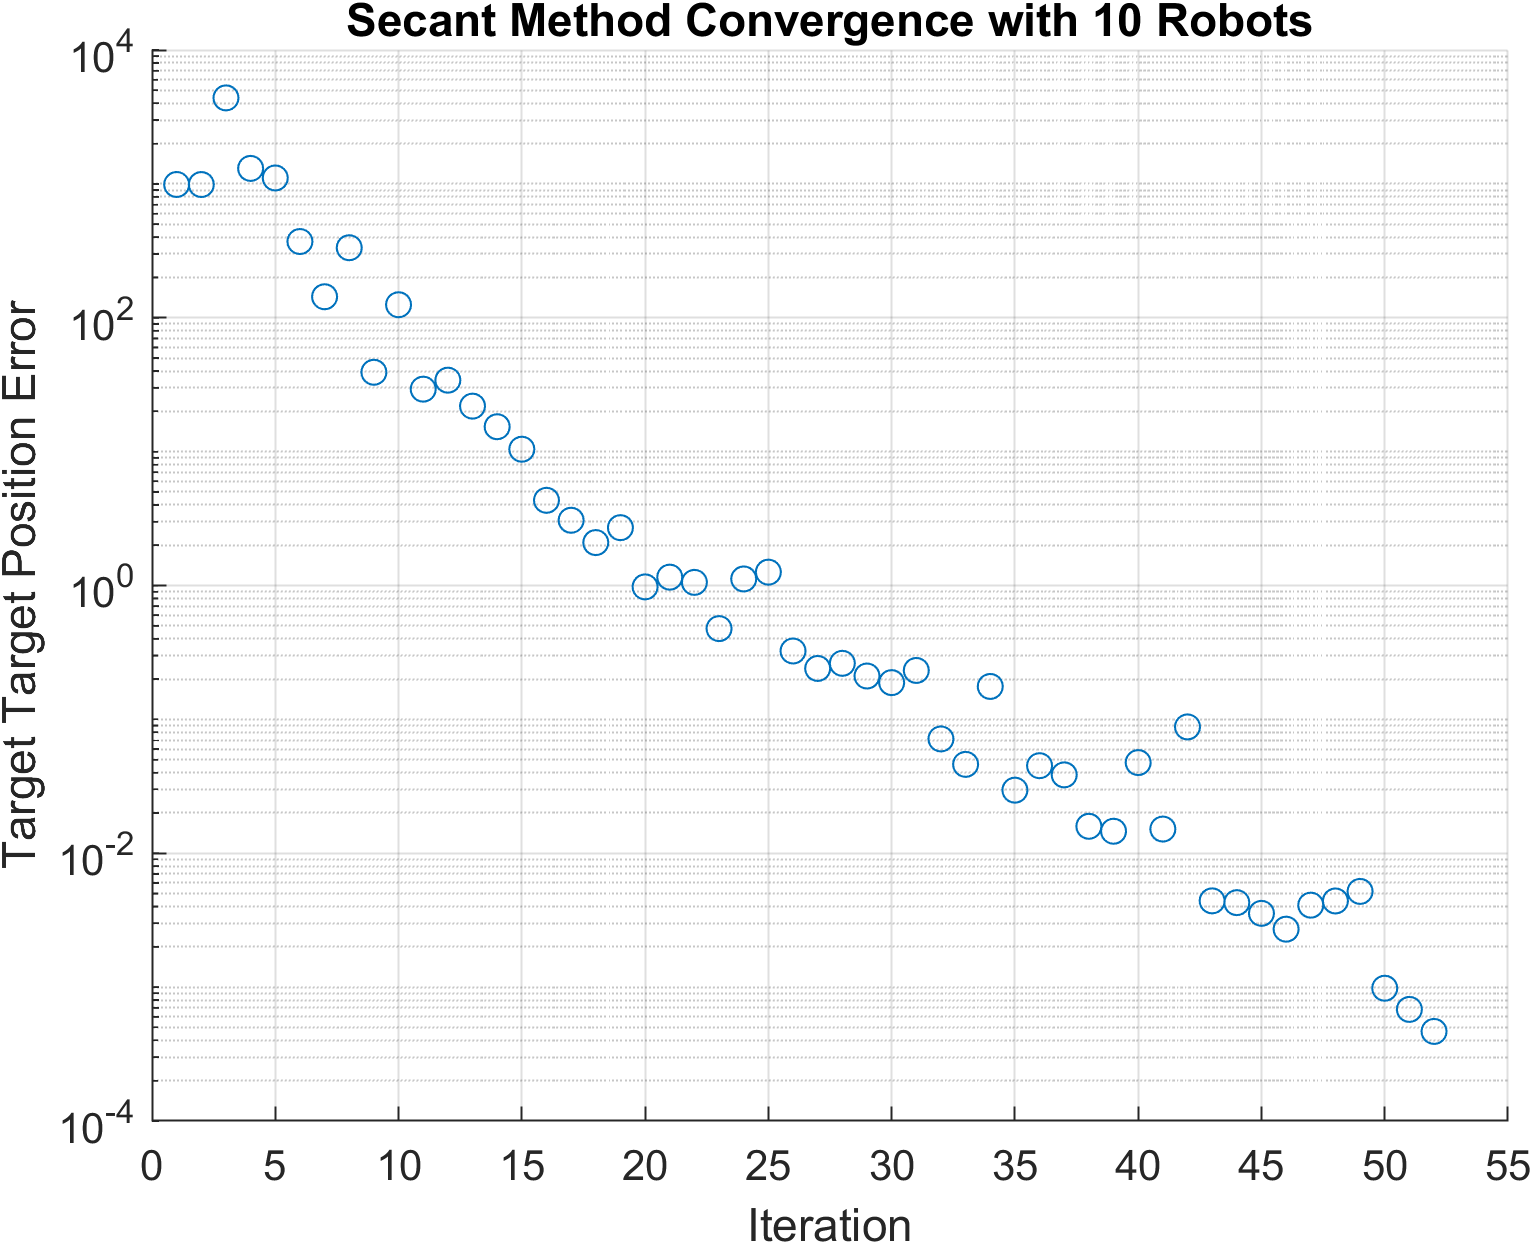
\includegraphics[width=0.7\linewidth]{N10M0_t_err}
	\caption{The total (sum of 10 robots) error between final trajectory position and target position for each iteration of secant method. 52 points evaluations are made as the first two initialization guesses are not included in the 50 total iterations, but their total errors are included.}
	\label{fig:n10m0-t-err}
\end{figure}

\begin{figure}
	\centering
	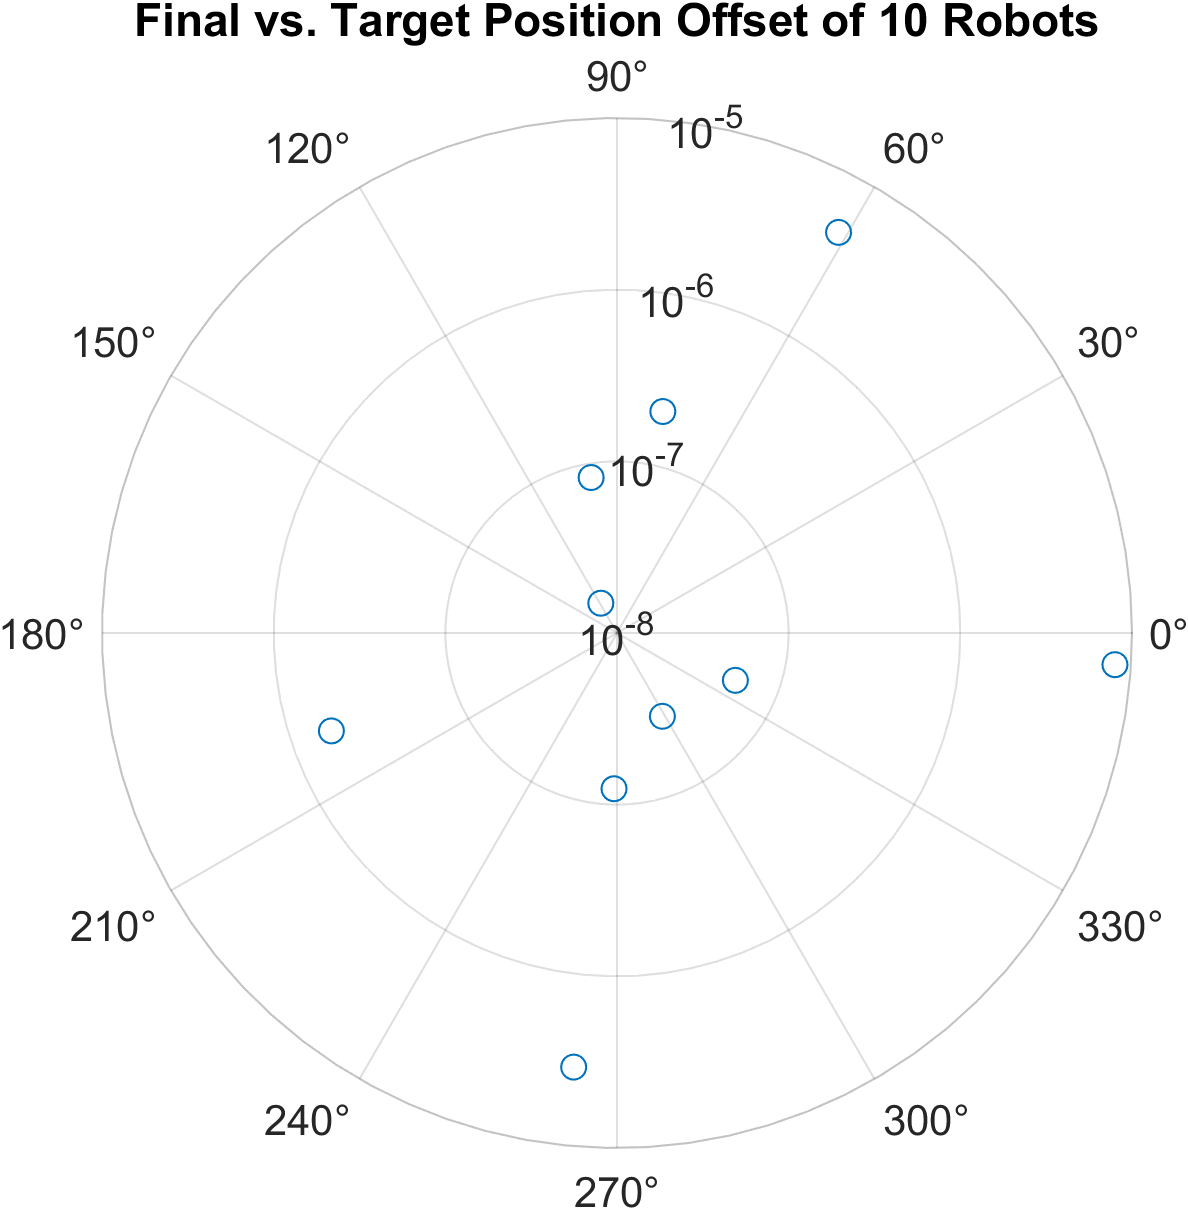
\includegraphics[width=0.5\linewidth]{N10M0_p_err}
	\caption{A log-polar graph of all target position errors for 10 robots.}
	\label{fig:n10m0-p-err}
\end{figure}

\clearpage

\subsection{Even More Robots!}

These same steps were repeated for 30 and 60 robots; their optimal trajectories, convergence of their total error, and their distribution of target position errors can be found in \Cref{fig:n30m0-paths,fig:n30m0-paths-zoom,fig:n30m0-t-err,fig:n30m0-p-err}.

Relatively good convergence was found for 30 robots, but exhibited plateaus in the first 30 iterations and the last 25. All target destinations were reached within a distance of 1 and curvature in the trajectories can be seen for close initial or target position pairs.

Unfortunately, due to the high dimensionality when there is 60 robots, the secant method was unable to converge, with some robots grossly overshooting their target positions by a magnitude greater than the space their restricted to. Other more robust or computationally efficient methods may be considered to combat this issue.

\begin{figure}
	\centering
	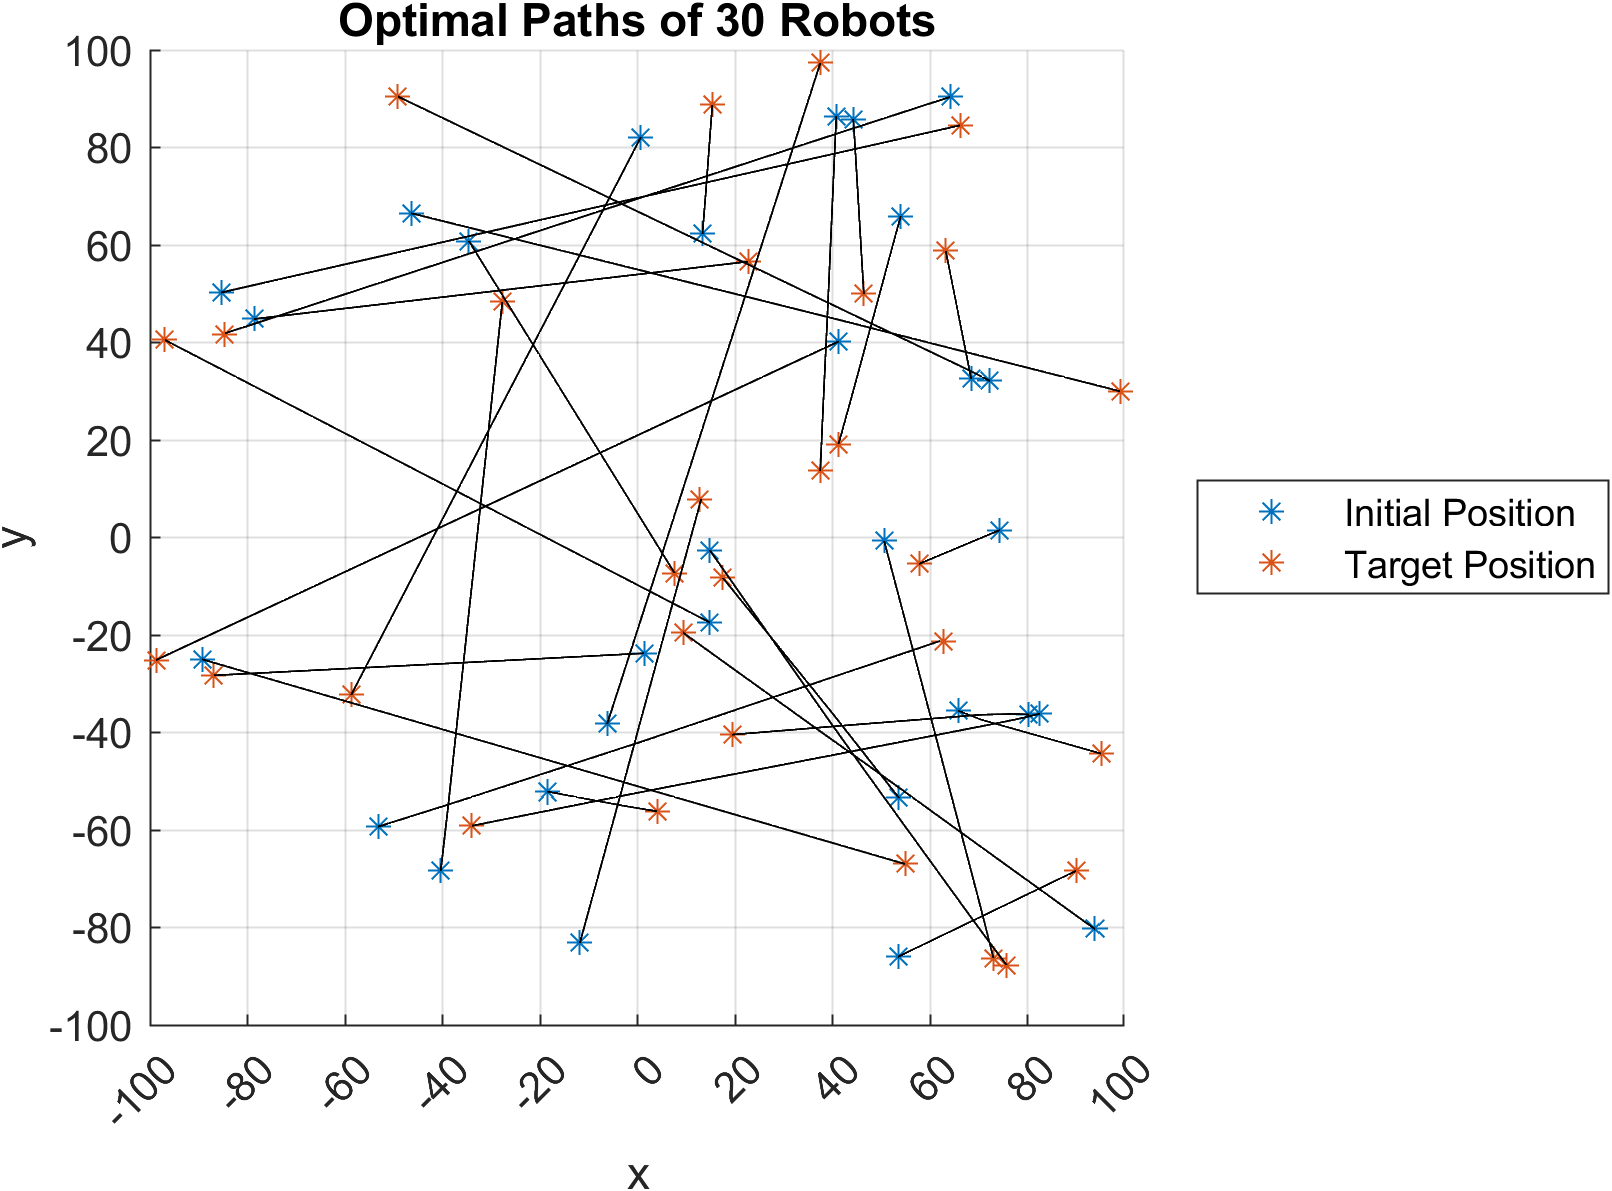
\includegraphics[width=0.75\linewidth]{N30M0_paths}
	\caption{Optimal trajectories for 30 robots and no obstacles placed uniformly at random. The trajectories were found using a shooting algorithm with the secant method.}
	\label{fig:n30m0-paths}
\end{figure}

\begin{figure}
	\centering
	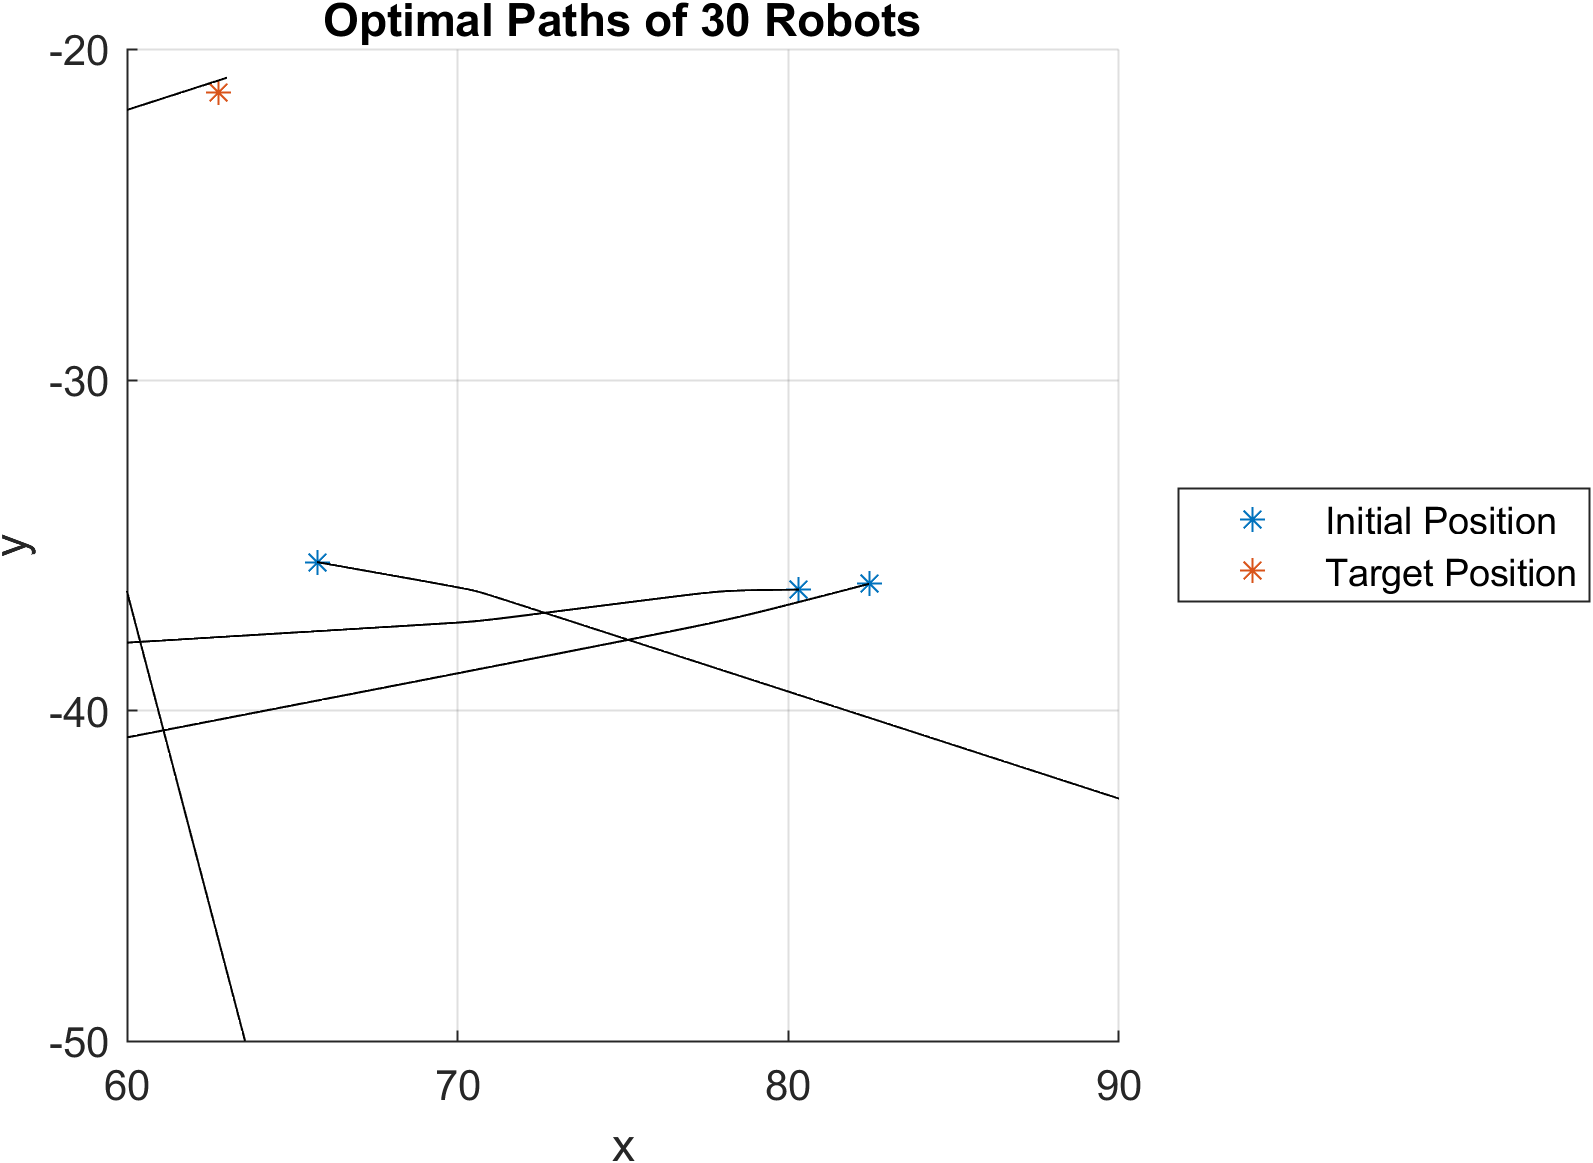
\includegraphics[width=0.75\linewidth]{N30M0_paths_zoom}
	\caption{The region \([60,90] \times [-50,-20]\) in \Cref{fig:n30m0-paths}. The curvature of the path can clearly be seen from two initial positions.}
	\label{fig:n30m0-paths-zoom}
\end{figure}

\begin{figure}
	\centering
	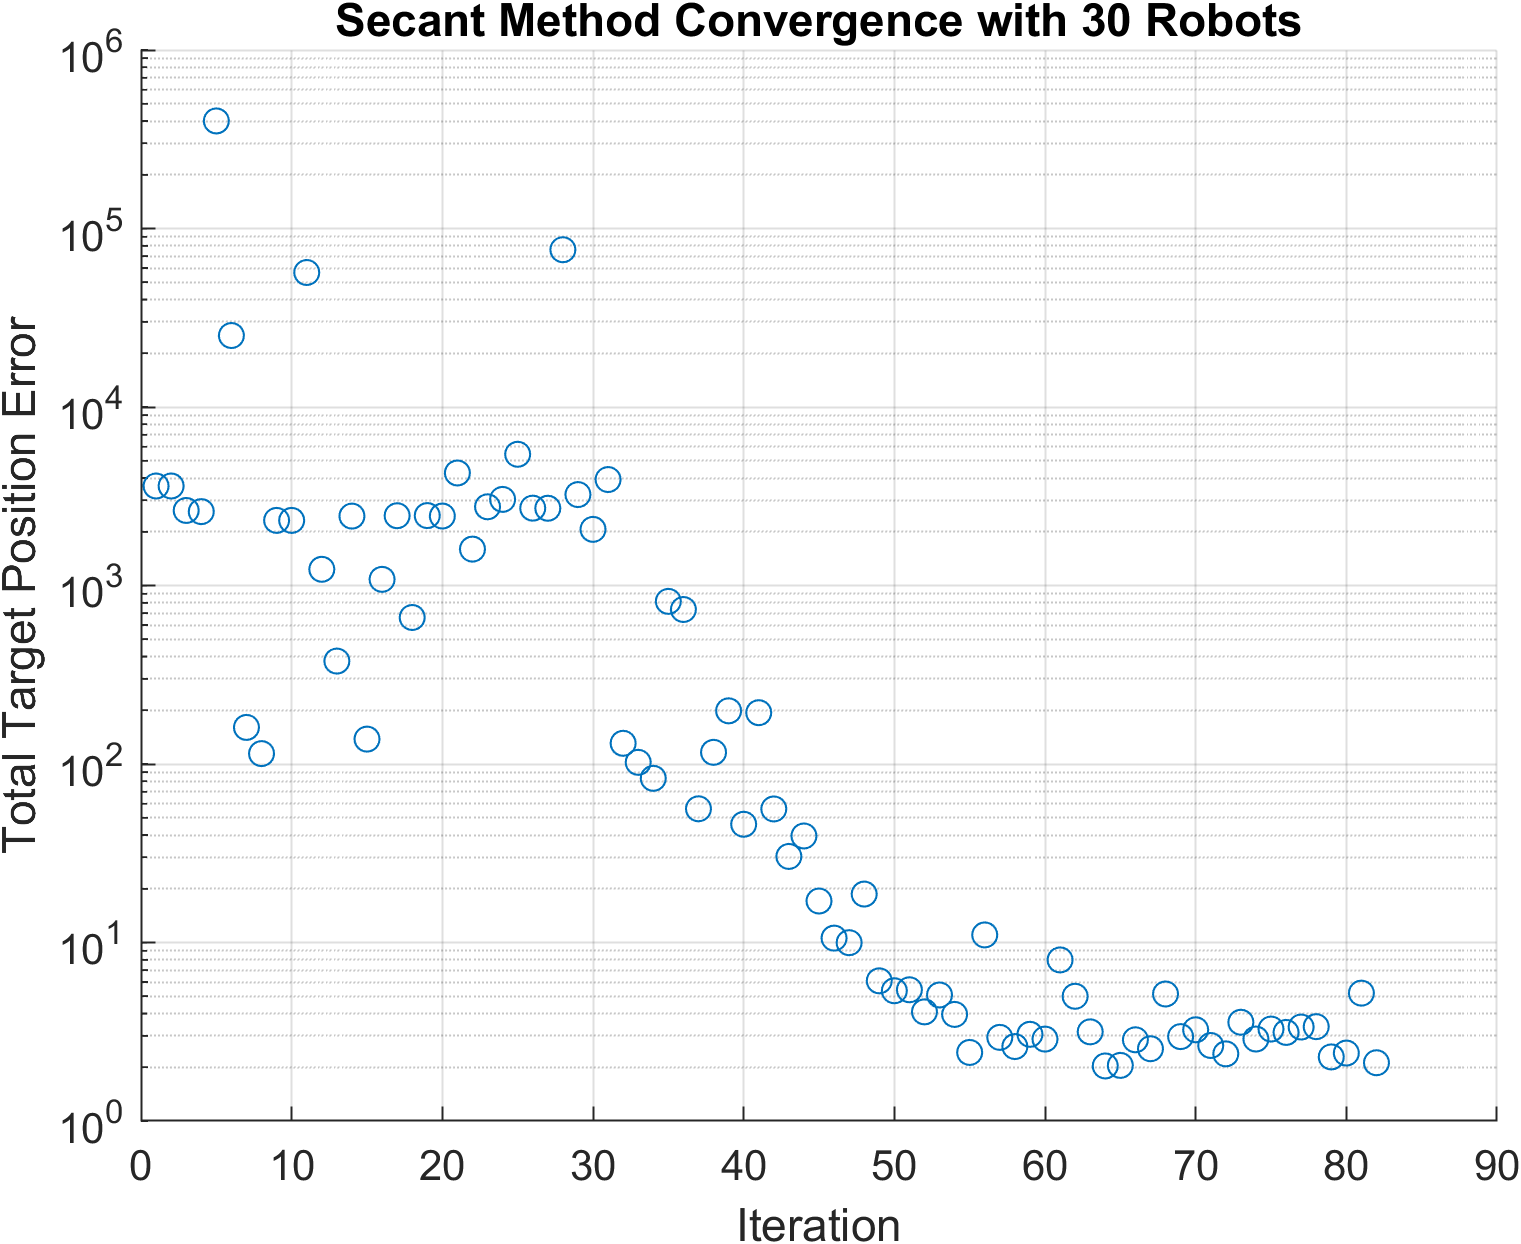
\includegraphics[width=0.7\linewidth]{N30M0_t_err}
	\caption{The total (sum of 30 robots) error between final trajectory position and target position for each iteration of secant method. 82 points evaluations are made as the first two initialization guesses are not included in the 80 total iterations, but their total errors are included.}
	\label{fig:n30m0-t-err}
\end{figure}

\begin{figure}
	\centering
	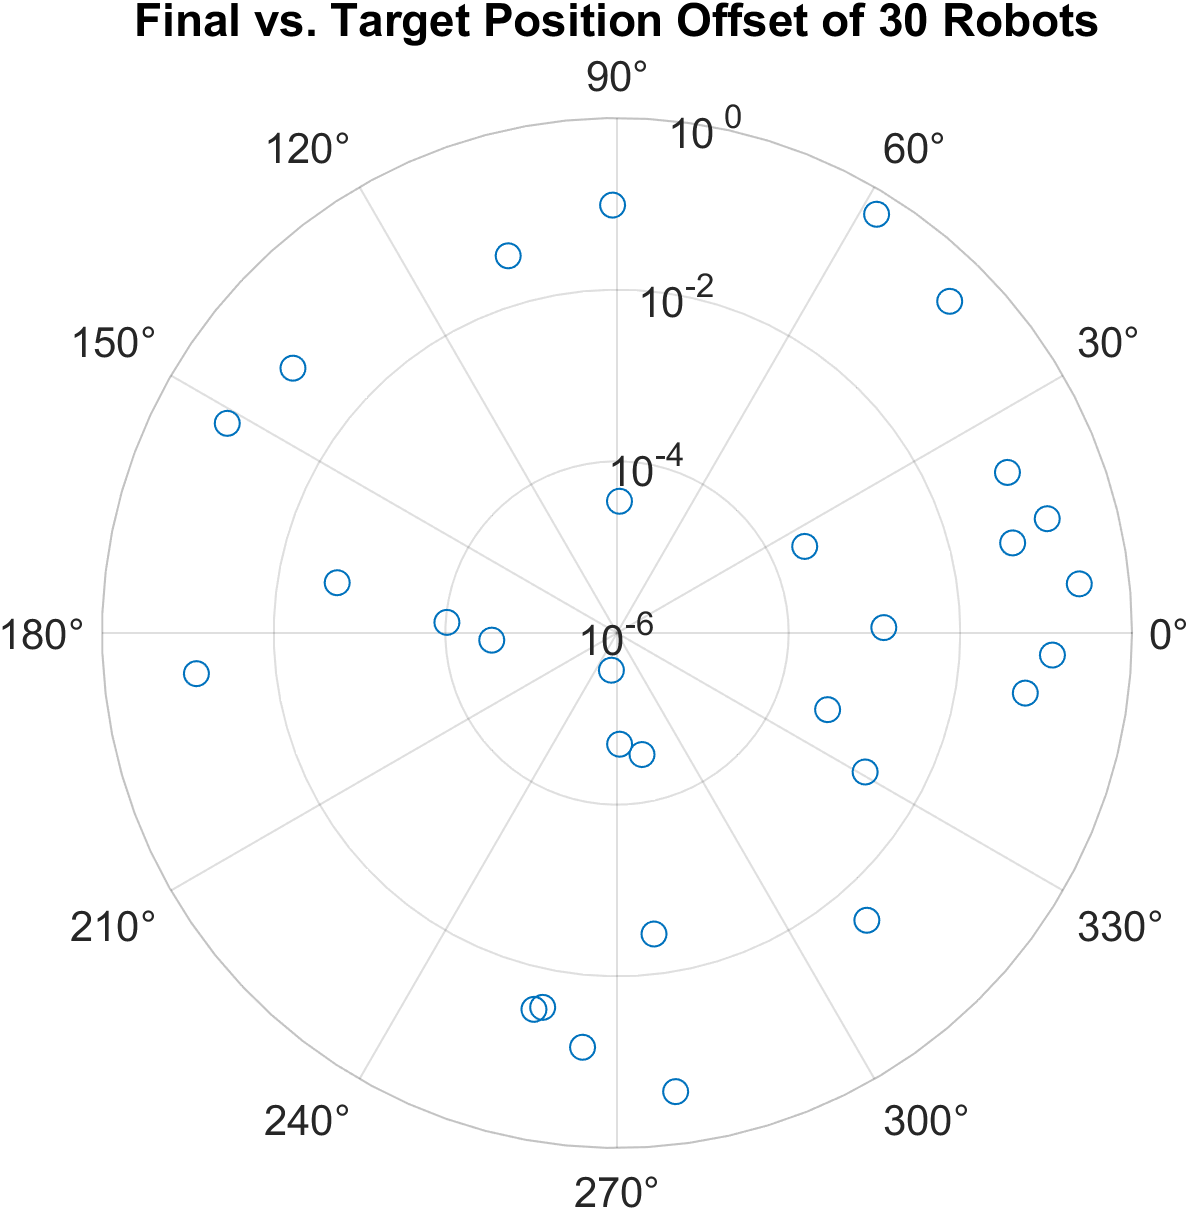
\includegraphics[width=0.5\linewidth]{N30M0_p_err}
	\caption{A log-polar graph of all target position errors for 30 robots.}
	\label{fig:n30m0-p-err}
\end{figure}

\begin{figure}
	\centering
	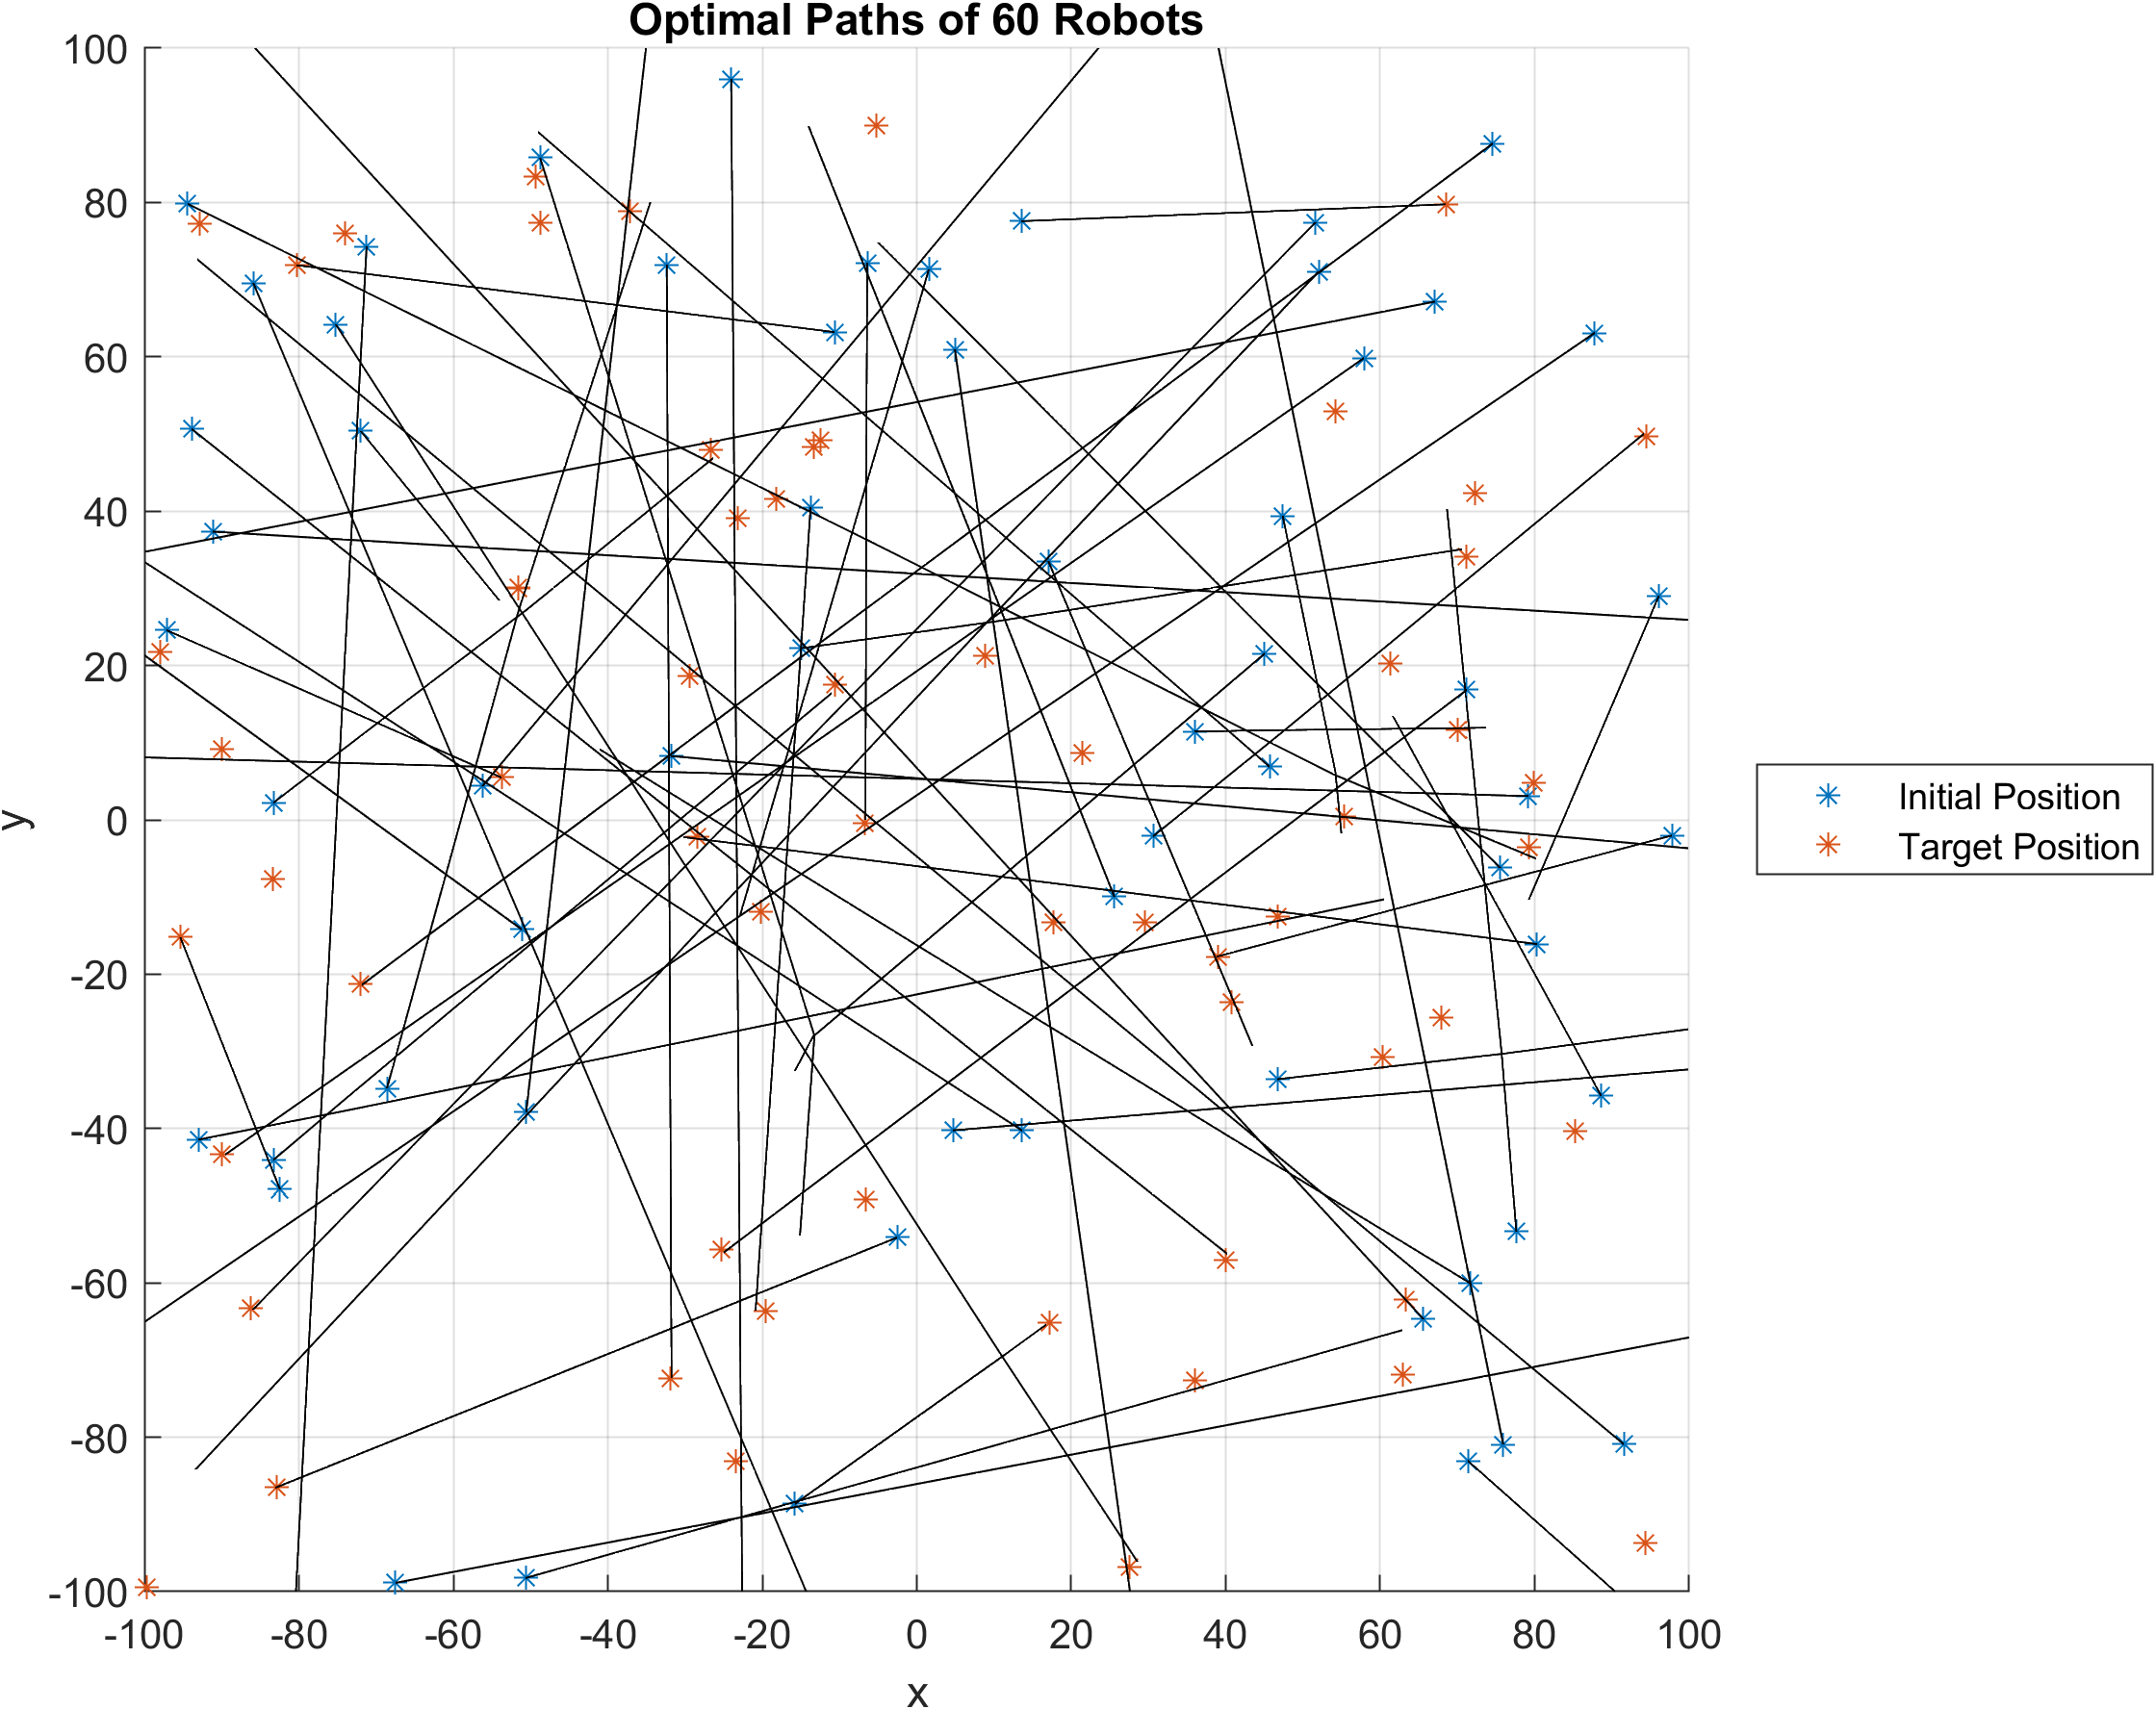
\includegraphics[width=0.9\linewidth]{N60M0_paths}
	\caption{Optimal trajectories for 60 robots and no obstacles placed uniformly at random. The trajectories were found using a shooting algorithm with the secant method.}
	\label{fig:n60m0-paths}
\end{figure}

\begin{figure}
	\centering
	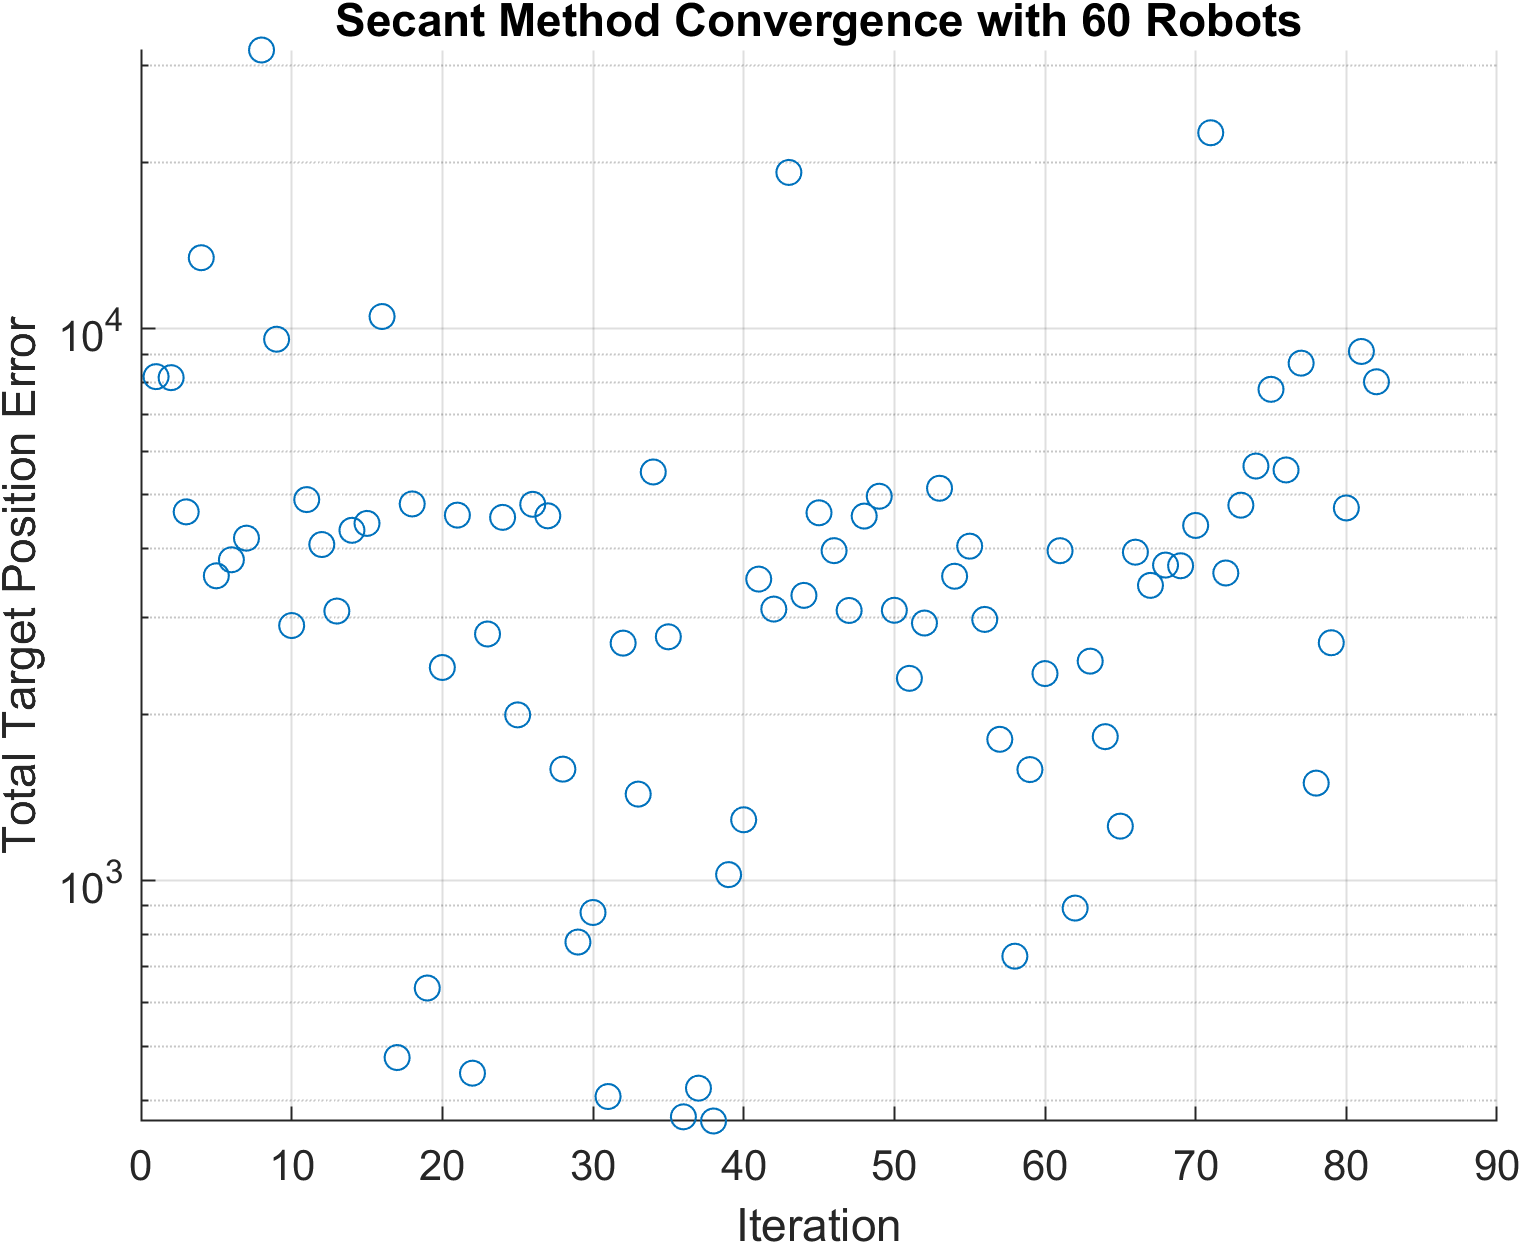
\includegraphics[width=0.7\linewidth]{N60M0_t_err}
	\caption{The total (sum of 60 robots) error between final trajectory position and target position for 80 iteration of secant method. Convergence is not seen due to high dimensionality of the search space.}
	\label{fig:n60m0-t-err}
\end{figure}

\begin{figure}
	\centering
	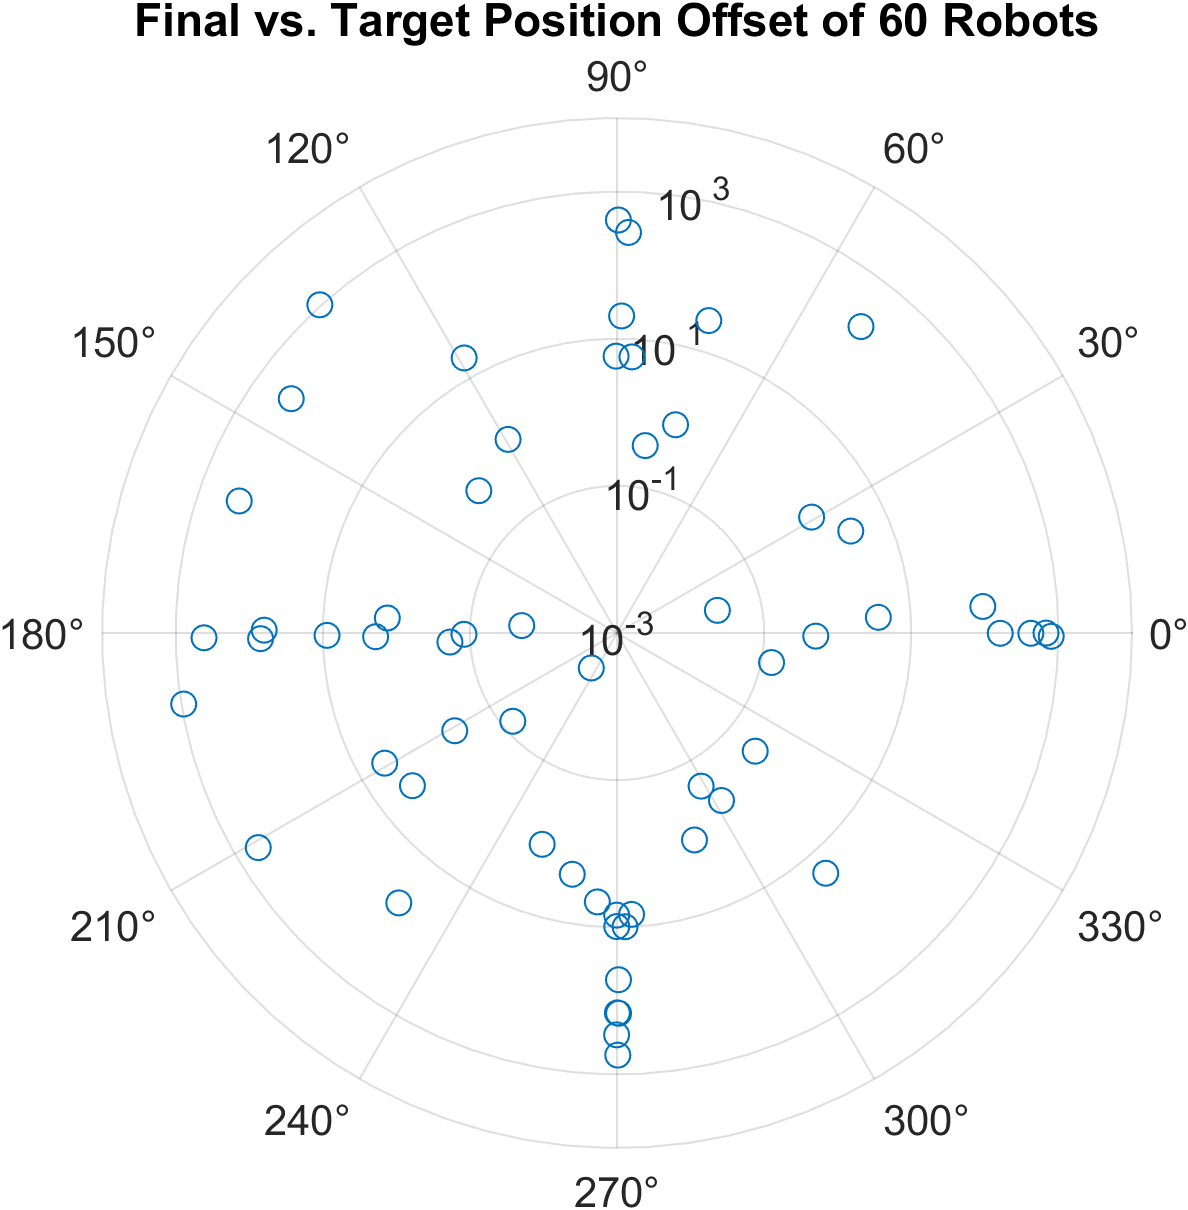
\includegraphics[width=0.5\linewidth]{N60M0_p_err}
	\caption{A log-polar graph of all target position errors for 60 robots.}
	\label{fig:n60m0-p-err}
\end{figure}

\section{Discussion}

\section{Conclusion}

\begin{appendices}

\section{MATLAB Code}

\end{appendices}

\end{document}

